\begin{enumerate}[label=\thesection.\arabic*.,ref=\thesection.\theenumi]
\numberwithin{equation}{enumi}
\item The number of directions and encirclements around the point -1+j0 in the complex plane by the Nyquist plot of $$G(s) = \frac{1-s}{4+2s}$$
\bigskip
\solution
First,we need to draw the polar plot of given G(S).
In the polar plot,substitute s = $j\omega$

\begin{align}
G(j\omega) = \frac{1-j\omega}{4+2j\omega} 
\end{align}

\begin{align}
\lim_{\omega\to\infty} G(j\omega) = \frac{1-j\omega}{4+2j\omega} 
\end{align}

\begin{align}
\lim_{\omega\to\infty} G(j\omega) = \frac{j\omega(\frac{1}{j\omega}-1)}{j\omega(\frac{4}{j\omega}+2)}  
\end{align}

\begin{align}
\lim_{\omega\to\infty} G(j\omega) = \frac{-1}{2}\angle 0  
\end{align}

which is equal to $\frac{1}{2}\angle{-180}$

As the Magnitude is taken positive in Nyquist Plot.
Now substitute $\omega = 0$

\begin{align}
\lim_{\omega\to\ 0} G(j\omega) = \frac{1-j\omega}{4+2j\omega} = \frac{1}{4}\angle 0 
\end{align}

so from this  at $\omega = 0$ $\angle G(j\omega) = 0$
and so from this  at $\omega = \infty$ $\angle G(j\omega)  =-180$     


\begin{align}
\mid(G(j\omega))\mid = \frac{\sqrt{1+{\omega}^2}}{\sqrt{16+{4\omega}^2}} 
\end{align}

when $\omega = 0$
\begin{align}
\mid(G(j\omega))\mid = \frac{1}{4}
\end{align}

when $\omega = \infty$
\begin{align}
\mid(G(j\omega))\mid = \frac{1}{2}
\end{align}


Hence,magnitude should be every time positive.
So,we have to plot first 0.25 then we have to turn {-180} degrees to that point i.e {180} degrees clockwise(in this case)
\bigskip

\item Now Plot the Polar Plot 1 from $\omega=0 to \infty$
\begin{figure}[!h]
  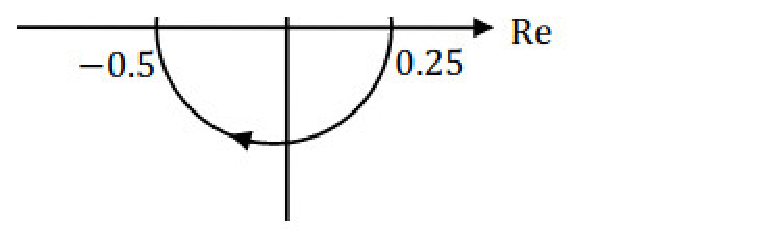
\includegraphics[width=\columnwidth]{./figs/image2.eps}
\end{figure}

\item Draw the Mirror image of the Polar Plot 1.
\begin{figure}[!h]
  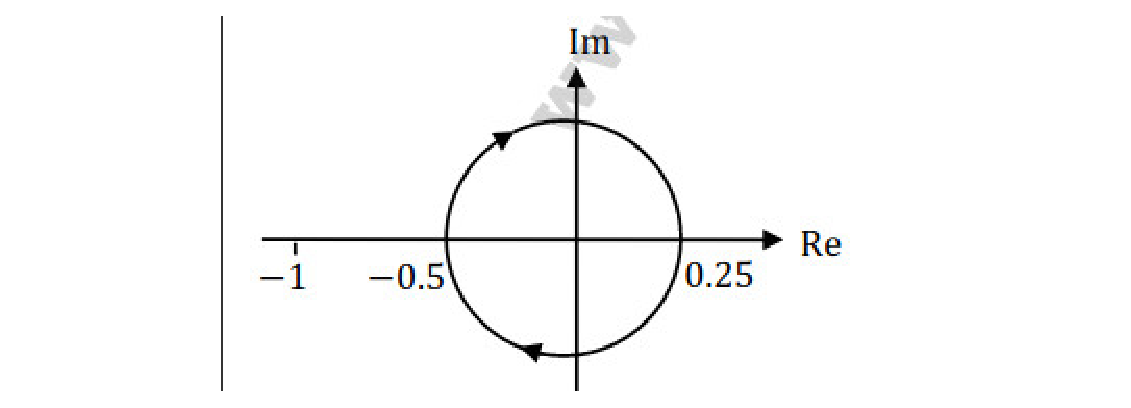
\includegraphics[width=\columnwidth]{./figs/image1.eps}
 
\end{figure}


\item Find the points where $G(j\omega)$ intersects the real and imaginary axes(if needed) and then locate the given co-ordinate




    $$Put\,s=Re^{j\theta}$$
    $$\lim_{R\to \infty}\,G(Re^{j\theta})=\frac{1-Re^{j\theta}}{4+2Re^{j\theta}}=\frac{-1}{2}$$ \\
    \bigskip
    As there are no $e^{j\theta}$ terms, 
    
    There there will be no enclosed Nyquist path here. 
    
    So, for this Transfer function $G(s)$,the Nyquist plot is same as the Polar plot.
    
\begin{figure}[!h]
  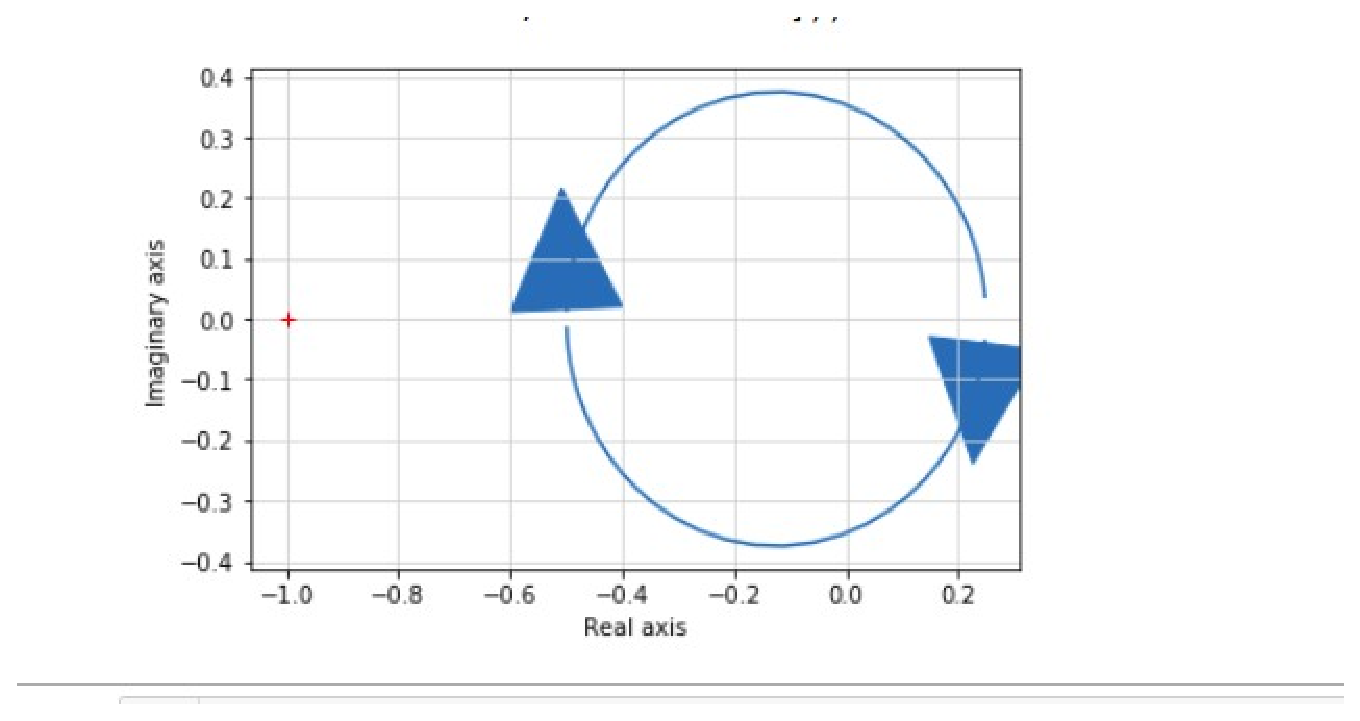
\includegraphics[width=\columnwidth]{./figs/pythonnyquistplot.eps}
 
\end{figure}




As from the observed plot the co-ordinate -1 + j0 is outside the contour

\bigskip

Hence,the number of encirclements around the the given co-ordinate is zero.



\end{enumerate}
